\documentclass[aspectratio=169]{beamer}

\usetheme{Madrid}
\usecolortheme{default}
\setbeamertemplate{navigation symbols}{}

\usepackage[T1]{fontenc}
\usepackage[utf8]{inputenc}
\usepackage{amsmath,amssymb}
\usepackage{booktabs}
\usepackage{graphicx}
\usepackage{array}

\title{Wavefront Detection for Tomography}
\subtitle{A geometry-aware learned primal-dual approach}
\author{Project presentation draft}
\date{\today}

\newcommand{\RP}{\mathbb{RP}^1}
\newcommand{\tY}{\tilde Y}
\newcommand{\G}{\mathcal G}
\newcommand{\bn}{\mathbf n}

\begin{document}

\begin{frame}
  \titlepage
\end{frame}

% ---------------------------------------------------------------------------
\begin{frame}{Goal In Plain Language}
  \begin{itemize}
    \item We estimate the \emph{wavefront set}: where the edges are and which direction they face.
    \item That means detecting oriented edges directly from tomographic data.
    \item We never compute a regularized or learned reconstruction. The data enter only through fixed linear filters, followed by a modulus.
    \item Hand-designed geometry is combined with a learned iterative solver.
  \end{itemize}
  \vspace{0.5em}
  \textbf{Why:} edges and directions are often more stable than intensities under tomography artifacts.
\end{frame}

\begin{frame}{What Is A Wavefront Set?}
  \begin{itemize}
    \item An edge map asks: \emph{is there an edge at this pixel?}
    \item A wavefront set also asks: \emph{which normal direction does it have?}
    \item So we work on a \textbf{lifted space} $(x,\theta)$: pixel $x$ and edge-normal angle $\theta$ (mod $\pi$ for real images).
  \end{itemize}
  \vspace{0.4em}
  \textbf{Plot convention:} a lifted field $u(x,\theta)$ is shown as one colour image,
  brightness $=\max_\theta u$, hue $=$ the maximising $\theta$.
  \begin{center}
    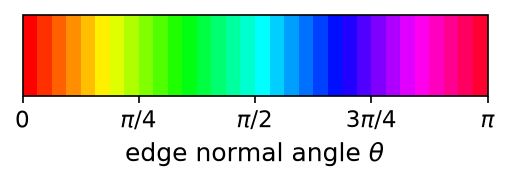
\includegraphics[width=0.32\linewidth]{assets/theta_legend.png}
  \end{center}
\end{frame}

\begin{frame}{Pipeline Overview}
  \centering
  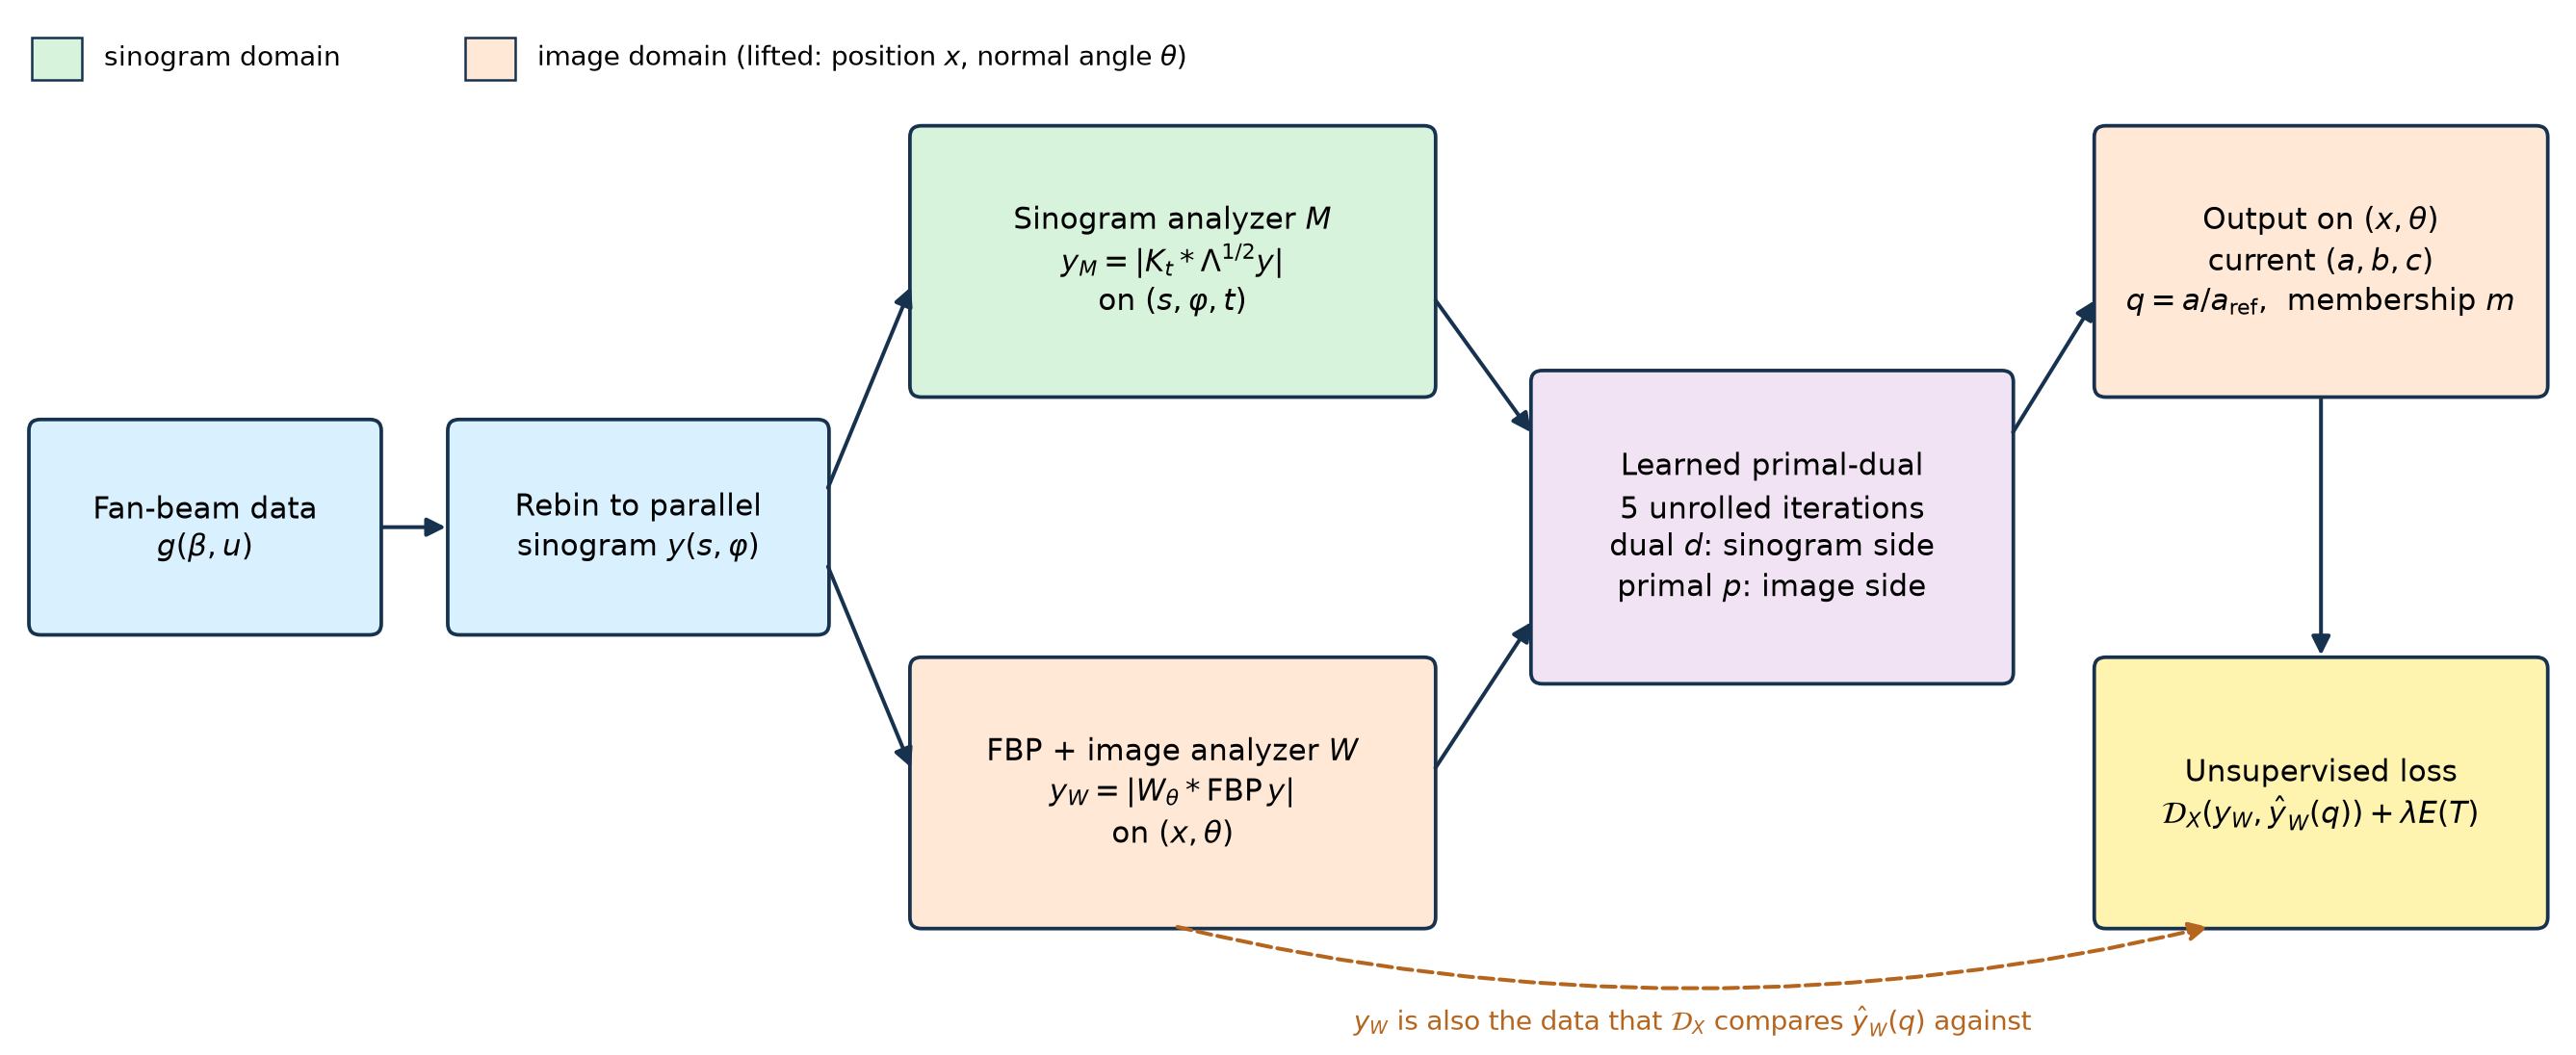
\includegraphics[width=0.93\linewidth]{assets/flowchart.png}

  \small The output and the data term live on the lifted image domain $(x,\theta)$. The LPD alternates between $\tY$ (dual) and $X$ (primal).
\end{frame}

% ---------------------------------------------------------------------------
\section{The building blocks}

\begin{frame}{The Canonical Relation}
  \centering
  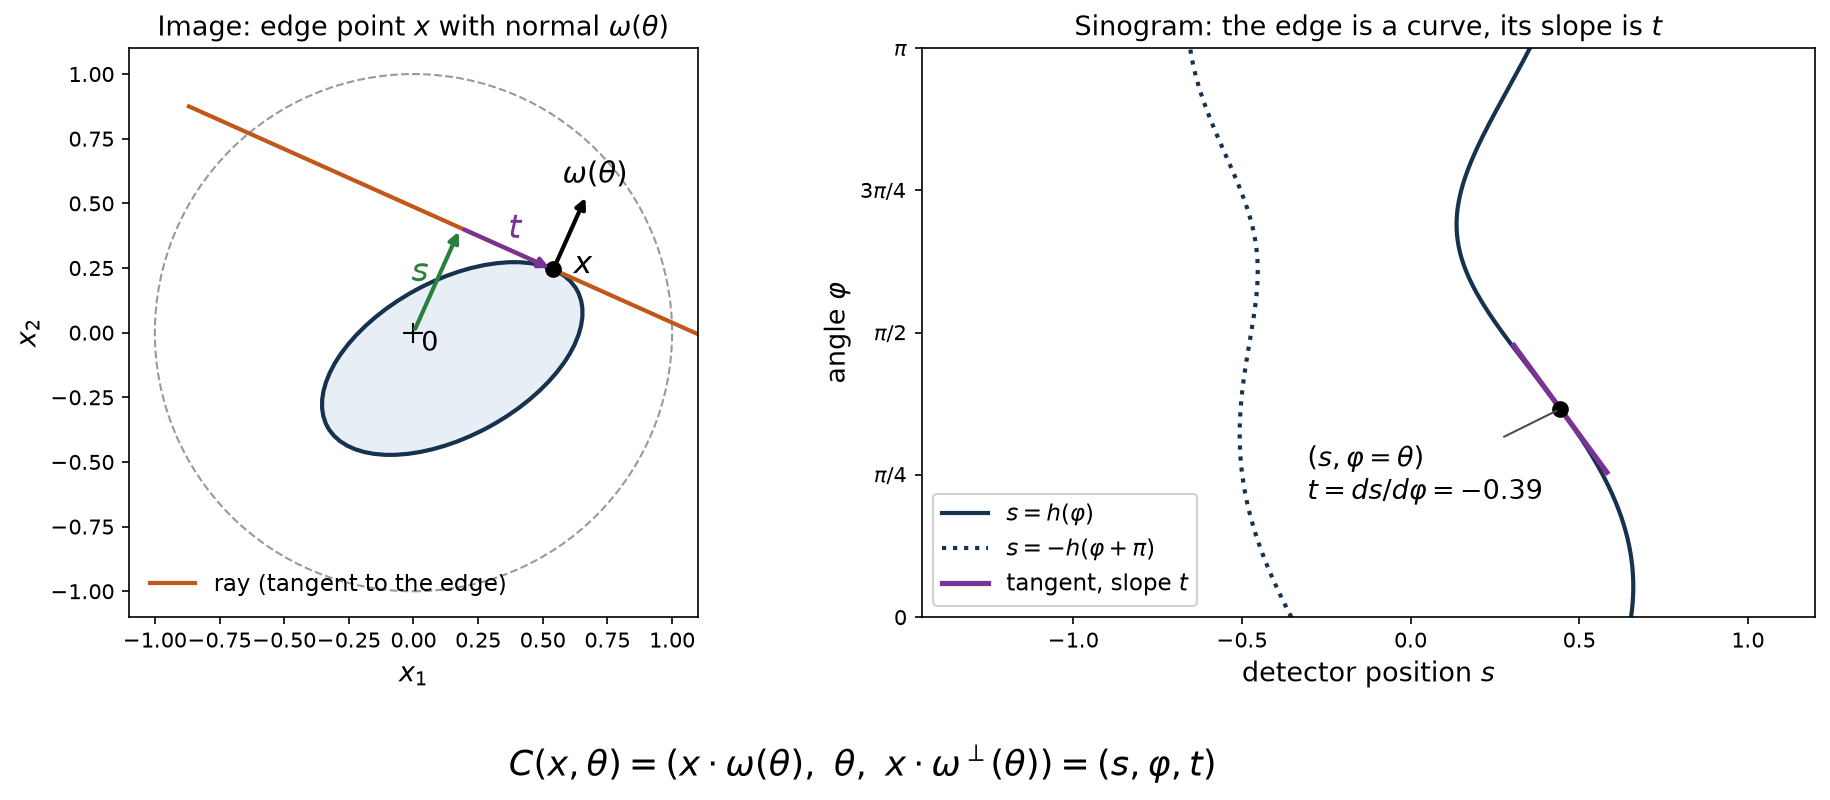
\includegraphics[width=0.72\linewidth]{assets/fig_canonical_relation.png}

  \small
  \begin{itemize}
    \item An edge point $(x,\theta)$ is seen by the ray tangent to the edge: $\mathrm{WF}(Rf)=C(\mathrm{WF}f)$.
    \item $t$ is the position of $x$ along that ray, and also the slope $ds/d\varphi$ of the sinogram curve.
    \item For each angle slice, $C$ is just a rotation of $x$ by $-\theta$.
  \end{itemize}
\end{frame}

\begin{frame}{Oriented Derivative-Of-Gaussian Filters}
  One generic kernel, for a unit normal $\bn$:
  \[
    \G_{\bn}(u)\propto u_\perp\,e^{-u_\perp^2/2\sigma_\perp^2-u_\parallel^2/2\sigma_\parallel^2},
    \qquad u_\perp=u\cdot\bn,\quad u_\parallel=u\cdot\bn^\perp .
  \]
  \begin{itemize}
    \item It differentiates across a curve with normal $\bn$ (width $\sigma_\perp$) and smooths along it (width $\sigma_\parallel$).
    \item $K*v$ means ``filter $v$ with $K$''.
    \item $|\cdot|$ is the pointwise magnitude of the signed response. It drops the sign of the jump (dark$\to$bright or bright$\to$dark), which the wavefront set ignores, and makes coefficients comparable with $q\ge0$.
    \item Cost of $|\cdot|$: edges in one filter (for $M$: on one ray) add \emph{before} the modulus.
    \item Both analyzers are instances: $K_t=\G_{\bn(t)}$ on $(s,\varphi)$ and $W_\theta=\G_{\omega(\theta)}$ on $x$.
  \end{itemize}
\end{frame}

\begin{frame}{Sinogram Analyzer $M$}
  \[
    y_M(s,\varphi,t)=\bigl|(K_t*\Lambda^{1/2}y)(s,\varphi)\bigr|,\qquad K_t=\G_{\bn(t)},\quad \bn(t)=\tfrac{(1,-t)}{\sqrt{1+t^2}}
  \]
  \centering
  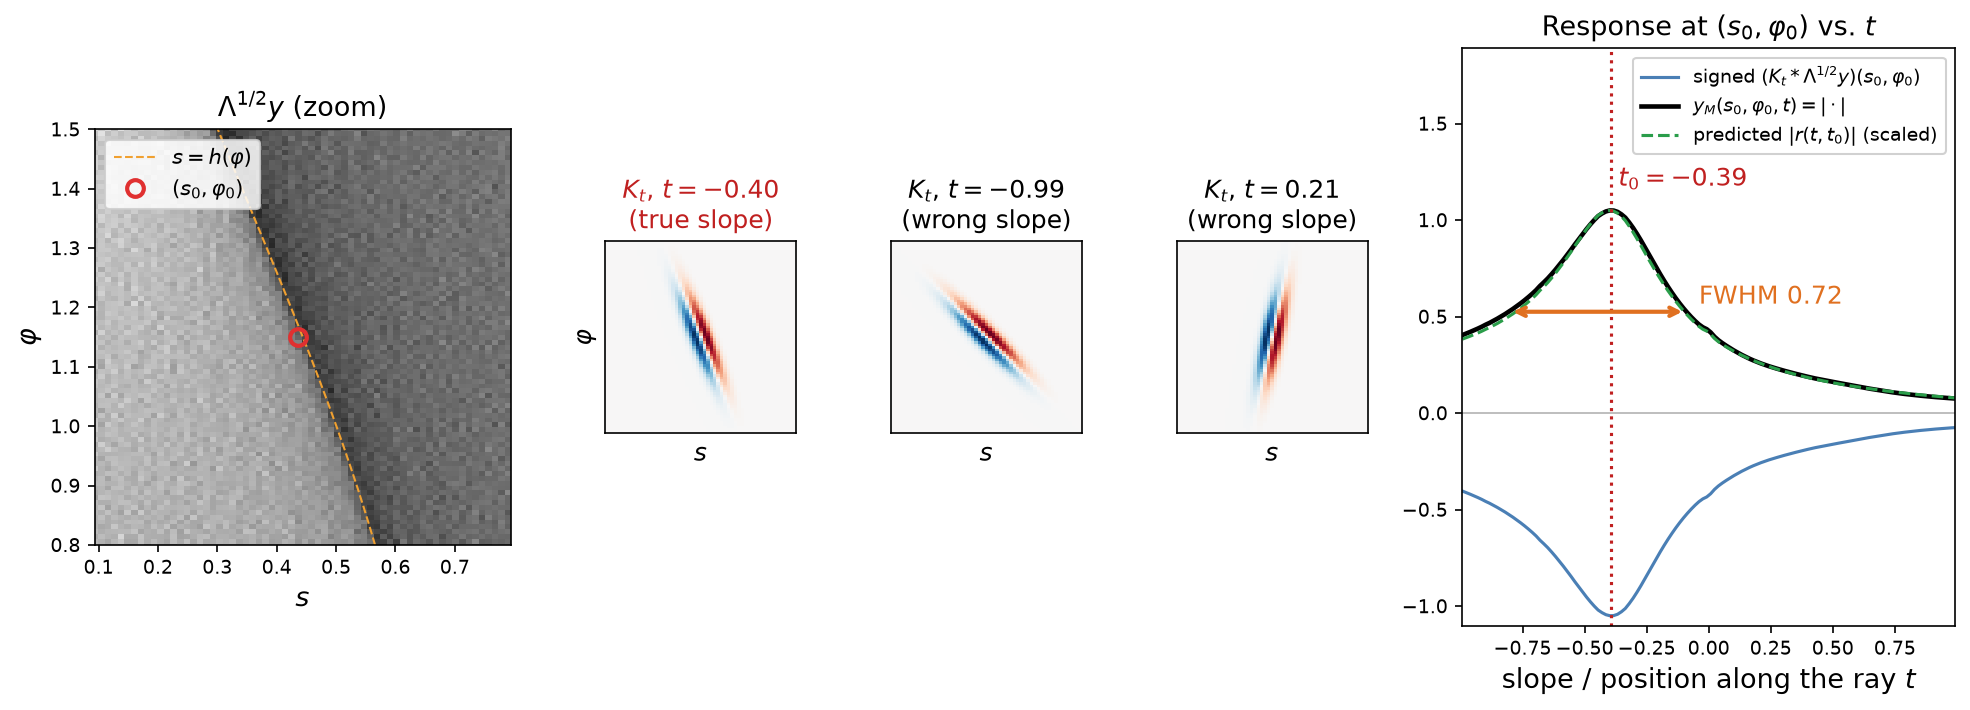
\includegraphics[width=0.86\linewidth]{assets/fig_sinogram_analyzer.png}

  \small\raggedright
  $\bn(t)$ is the normal of a sinogram curve of slope $t$, so $K_t$ responds most where the slope matches.
  $\Lambda^{1/2}$ (half ramp) turns curved-edge singularities into jumps. Aspect $\sigma_\parallel=6\sigma_\perp$.
\end{frame}

\begin{frame}{Limitation Of $M$: Poor Resolution In $t$}
  \begin{columns}[T]
    \begin{column}{0.45\linewidth}
      \begin{itemize}
        \item The response along $t$ is wide: FWHM $\approx0.72$ in $t$ for the ellipse on the last slide (positions lie in $|t|\le1$).
        \item Pulled back by $C^{-1}$, each edge point becomes a \textbf{streak along its tangent line}.
        \item Longer kernels do not help: sinogram curves are curved.
      \end{itemize}
    \end{column}
    \begin{column}{0.53\linewidth}
      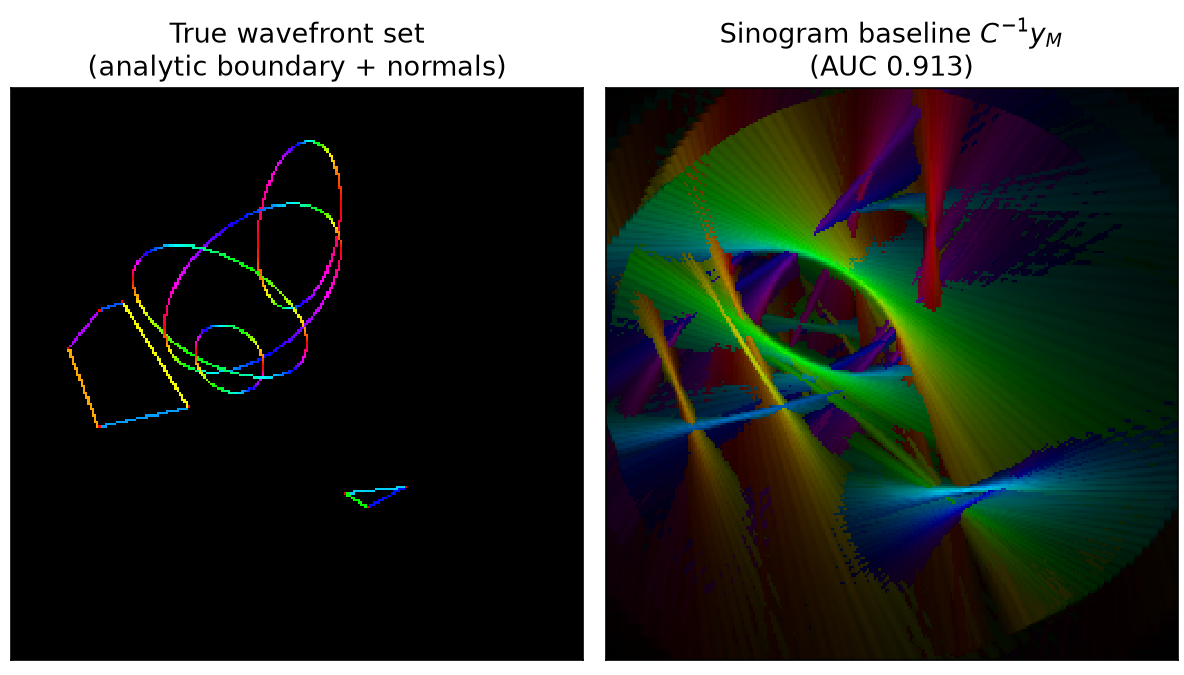
\includegraphics[width=\linewidth]{assets/fig_streaks.png}
    \end{column}
  \end{columns}
\end{frame}

\begin{frame}{Image Analyzer $W$}
  \[
    y_W(x,\theta)=\bigl|(W_\theta*\mathrm{FBP}\,y)(x)\bigr|,\qquad W_\theta=\G_{\omega(\theta)},\quad \sigma_\perp=1.5\text{ px},\ \sigma_\parallel=3\text{ px}
  \]
  \begin{itemize}
    \item FBP combines all angles, so the position along the ray is resolved.
    \item $K=32$ orientation slices; Hann-filtered FBP.
    \item Edge of contrast $h$ at distance $d$: $y_W\approx h\,|r_\theta(\theta,\theta_e)|\,e^{-d^2/2\sigma_e^2}$, $\sigma_e\approx2.6$ px. The data term uses this response.
    \item \textbf{Trade-off:} sharp in $x$, broad in angle (angular FWHM $\approx 83^\circ$).
    \item Still a fixed linear map of $y$, then $|\cdot|$ (identity in the backup slide).
  \end{itemize}
\end{frame}

\begin{frame}{Where Does Each Quantity Live?}
  \begin{columns}[T]
    \begin{column}{0.5\linewidth}
      \textbf{Sinogram side} $\tY\ni(s,\varphi,t)$
      \begin{itemize}
        \item data $y(s,\varphi)$
        \item coefficients $y_M=|My|$
        \item LPD dual variable $d$
      \end{itemize}
    \end{column}
    \begin{column}{0.5\linewidth}
      \textbf{Image side} $X\ni(x,\theta)$
      \begin{itemize}
        \item coefficients $y_W=|W_\theta*\mathrm{FBP}\,y|$
        \item LPD primal variable $p$
        \item outputs $a,b,c$ (the current $T$), $q=a/a_\mathrm{ref}$, $m$
      \end{itemize}
    \end{column}
  \end{columns}
  \vspace{0.6em}
  \[
    (C^{-1}y_M)(x,\theta)=y_M\bigl(x\cdot\omega,\,\theta,\,x\cdot\omega^\perp\bigr).
  \]
  The output $q$ lives on the image domain. In training, the data term $\mathcal D_X$ uses $y_W$; $y_M$ is only a network input.\footnote{Fields are stored on $Y$ and $X'$ ($\theta,\varphi\in[0,\pi)$); the network computes on the double covers $\tY$ and $X$.}
\end{frame}

\begin{frame}{The Network: Learned Primal-Dual}
  \begin{columns}[T]
    \begin{column}{0.52\linewidth}
      \begin{itemize}
        \item Inputs: $y_M$ (sinogram side) and $y_W$ (image side).
        \item 5 unrolled primal-dual iterations.
        \item Small CNNs $\Gamma_i,\Lambda_i$ (24 channels).
        \item $C$ and $C^{-1}$ move information between the two sides.
      \end{itemize}
    \end{column}
    \begin{column}{0.46\linewidth}
      \[
      d_{i+1}=d_i+\Gamma_i([d_i,Cp_i,y_M])
      \]
      \[
      p_{i+1}=p_i+\Lambda_i([p_i,C^{-1}d_{i+1},y_W])
      \]
      \vspace{0.4em}
      \begin{block}{Interpretation}
      The dual state checks consistency with the sinogram data. The primal state holds the current oriented-curve estimate.
      \end{block}
    \end{column}
  \end{columns}
\end{frame}

\begin{frame}{Network Outputs}
  \begin{itemize}
    \item The readout gives the current $(a,b,c)$ directly on $(x,\theta)$; no separate edge detection is needed.
    \item Amplitude $q=a/a_\mathrm{ref}$ enters the data term: $a\ge0$ is the line density, proportional to edge strength.
    \item $a_\mathrm{ref}=1/(2\pi\sigma_x\sigma_\theta)$, $\sigma=2$ cells: the peak line density of a resolved unit curve, so $q=1$ predicts a unit edge. A fixed normalization, not tuned.
    \item Membership $m=1-e^{-q}\in[0,1)$: for display and thresholds only.
    \item No separate contrast output (backup slide).
    \item Ridge extraction (non-maximum suppression) is used only to evaluate thin curves.
  \end{itemize}
\end{frame}

\begin{frame}{Training Objective}
  \[
    \min_{\text{network}}\ \mathbb{E}_{\text{data}}\bigl[\, \mathcal D_X(y_W,\hat y_W) + \lambda\, E(T)\bigr], \qquad \lambda=10^{-4}
  \]
  \textbf{Forward model:} predict the image coefficients from $q=a/a_\mathrm{ref}$,
  \[
    \hat y_W=F_X(q)=\tfrac{1}{w_X}\,G *_x \Bigl(\textstyle\sum_{\theta'} |r_\theta(\theta,\theta')|\;q(x,\theta')\Bigr)
  \]
  \textbf{Data term:} robust misfit, $\mathcal D_X=\operatorname{mean}_{x,\theta}\ \bigl|y_W-\hat y_W\bigr|_\delta$, \ $|e|_\delta=\sqrt{e^2+\delta^2}-\delta$.
  \begin{itemize}
    \item $r_\theta$: angular response of $W$; $G$: small Gaussian; $w_X$: unit curve $\mapsto\hat y_W=1$.
    \item \textbf{Unsupervised}: no labels. Labels are used only for validation.
  \end{itemize}
\end{frame}

\begin{frame}{What Should The Prior Do? Five Desiderata}
  A prior $P(T)\propto e^{-\lambda E(T)}$ on unions of curves $T=\sum_k T_k$ should give:
  \vspace{0.5em}
  \begin{center}
  \small
  \renewcommand{\arraystretch}{1.25}
  \begin{tabular}{@{}>{\raggedright}p{0.30\linewidth}>{\raggedright}p{0.40\linewidth}>{\raggedright\arraybackslash}p{0.22\linewidth}@{}}
    \toprule
    \textbf{desideratum} & \textbf{what $E$ guarantees} & \textbf{provided by} \\
    \midrule
    1.\ independent components: $P(T)=\prod_k P(T_k)$ & $E$ is additive over disjoint curves & local integrals \\
    2.\ smoothness & penalizes total turning, $\int\!\sqrt{1+\ell_\theta^2\kappa^2}\,ds$; corners allowed & turning term $\ell_\theta\,b$ \\
    3.\ stability: breaking a curve is unlikely & a gap of length $\varepsilon$ costs $2\nu-\varepsilon>0$ & endpoint term $\nu$ \\
    4.\ closed curves are favoured & closed curves have no boundary, $\partial T=0$ & endpoint term $\nu$ \\
    5.\ sparsity & (for curves) every component costs at least $\min(2\nu,\,2\pi\ell_\theta)$ & length + endpoints \\
    \bottomrule
  \end{tabular}
  \end{center}
  \vspace{0.3em}
  \small Rows 1--4: Prop.~3.7; row 5: Thm.~3.8, for curves only.
\end{frame}

\begin{frame}{The Current $T$}
  \textbf{$T$ is the wavefront set written as a 1-current} on $(x,\theta)$:
  \[
    T=\tau\,dX,\qquad \tau = a\,X_1 + b\,X_3 + c\,X_2,
  \]
  \[
    X_1=(-\sin\theta,\cos\theta,0)\ \text{(tangent)},\quad X_2=(\cos\theta,\sin\theta,0)\ \text{(normal)},\quad X_3=\partial_\theta\ \text{(turning)}.
  \]
  \begin{itemize}
    \item $a\ge0$: line density (gives $m$).
    \item $b=a\kappa$: rate of turning.
    \item $c$: non-physical ``sideways'' motion. Blurring creates it (Prop.~6.2), so it is kept, and penalized.
  \end{itemize}
\end{frame}

\begin{frame}{The Energy $E(T)$}
  \[
    E(T)=\underbrace{\int\!\sqrt{a^2+\ell_\theta^2 b^2+\zeta^2c^2}\;dX}_{\text{length (Riemannian approx.\ of sub-Riemannian)}}
    \;+\;\nu\underbrace{\int\!\bigl|X_1a+X_3b+X_2c\bigr|\,dX}_{|\mathrm{div}\,\tau|:\ \text{endpoints}}
  \]
  \begin{itemize}
    \item $a$: total edge length $\to$ sparsity (row 5).
    \item $\ell_\theta b$: turning cost, $\ell_\theta=0.3$ $\to$ smoothness with corners (row 2).
    \item $\zeta c$: keeps $\theta$ equal to the curve normal, $\zeta=2$ (Legendrian condition).
    \item $\nu|\mathrm{div}\,\tau|$: each open end costs $\nu=0.5$ $\to$ stability, closure (rows 3, 4).
    \item Local integrals $\to$ independence (row 1).
  \end{itemize}
\end{frame}

\begin{frame}{Why Not A Simpler Regularizer? (1/2)}
  \begin{itemize}
    \item \textbf{Plain length / TV on $m$:} independence and sparsity only. Length alone \emph{rewards} a gap (it saves $\varepsilon$). The endpoint term makes a gap cost $2\nu-\varepsilon>0$.
    \item \textbf{Curvature in the image plane} ($\int\kappa^2\,ds$) is second order and non-convex on pixels. On $(x,\theta)$, turning is \emph{first order} ($\partial_\theta$), so $E$ is \textbf{convex} in $\tau$.
    \item $\hat y_W$ is linear in $q=a/a_\mathrm{ref}$ and the misfit is convex, so the whole MAP objective is \textbf{convex} in $\tau$.
  \end{itemize}
\end{frame}

\begin{frame}{Why Not A Simpler Regularizer? (2/2)}
  \begin{itemize}
    \item \textbf{Orientation consistency:} $\zeta c$ ties $\theta$ to the actual curve direction. Without it, $\theta$ is a free label per pixel.
    \item \textbf{Euler elastica} ($\int\alpha+\beta\kappa^2\,ds$) forbids corners. Here a corner costs only $\ell_\theta\cdot$angle.
    \item \textbf{Few knobs:} $\ell_\theta$ (turning scale), $\zeta$ (orientation), $\nu$ (endpoints).
    \item Gaps shorter than $2\nu$ are bridged; $2\nu=1$ is the radius of the object disk, so $\nu$ acts as an endpoint penalty.
  \end{itemize}
\end{frame}

% ---------------------------------------------------------------------------
\section{Results}

\begin{frame}{Ground Truth And Baselines (Synthetic Phantoms)}
  \begin{itemize}
    \item \textbf{True wavefront set:} analytic, from the phantom shapes (ellipses, polygons): boundary samples with outward normal $\theta$, rasterised to $256^2\times64$. Corners get all angles.
    \item \textbf{Sinogram baseline $C^{-1}y_M$:} learning-free, $y_M$ pulled back by $C^{-1}$.
    \item \textbf{Image baseline $y_W$:} learning-free, oriented filters on the FBP.
    \item \textbf{LPD $m$:} the network's membership output.
  \end{itemize}
\end{frame}

\begin{frame}{Metric 1: ROC AUC}
  \[
    \mathrm{AUC}=P\bigl(\text{score}(v^+)>\text{score}(v^-)\bigr)\qquad\text{(Mann--Whitney)}
  \]
  \begin{itemize}
    \item $v^+$, $v^-$: random positive and negative lifted voxels.
    \item Positives: soft label $\ge0.5$. Negatives: soft label $<0.01$. Voxels in between are ignored (a gap).
    \item \textbf{Why:} threshold-free, and it ranks every voxel.
  \end{itemize}
\end{frame}

\begin{frame}{Metric 2: Thin-Ridge Precision, Recall And F}
  \begin{itemize}
    \item Ridges: keep $(x,\theta)$ if $u$ is a local max across the edge (along $\pm\omega(\theta)$) and in $\theta$, and $u\ge\eta\max u$.
    \item $P=\dfrac{\#\text{matched predicted ridge points}}{\#\text{predicted}}$,\quad
          $R=\dfrac{\#\text{matched true points}}{\#\text{true}}$,\quad
          $F=\dfrac{2PR}{P+R}$.
    \item Match within $1.5$ px and $\pm1$ $\theta$ bin. ODS: one best $\eta$ for the whole dataset.
    \item $F_x$: the same, spatial only (ignores $\theta$).
    \item \textbf{Why:} we want thin curves with the correct orientation.
  \end{itemize}
\end{frame}

\begin{frame}{Why AUC Alone Is Misleading Here}
  \begin{columns}[T]
    \begin{column}{0.50\linewidth}
      \small
      \begin{itemize}
        \item Imbalance: positives are $0.26\%$ of voxels, negatives $98.3\%$ (sample 0).
        \item $C^{-1}y_M$ there: at the median positive score, only $1.30\%$ of negatives score higher, yet that is ${\approx}\,10$ false voxels per detected true one (precision ${\approx}\,9\%$). AUC is still $0.937$.
        \item The $\max_\theta$ display exaggerates the streaks.
        \item Complements: \textbf{AP} (area under the PR curve), and \textbf{hard-negative AUC} (negatives within 6 px of the true edges).
      \end{itemize}
    \end{column}
    \begin{column}{0.48\linewidth}
      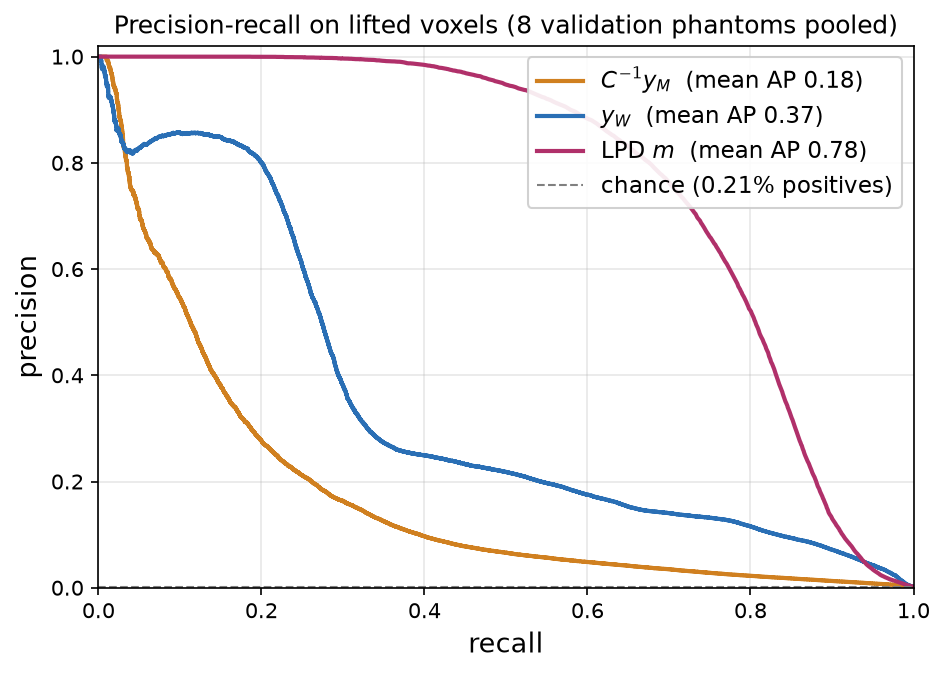
\includegraphics[width=\linewidth]{assets/fig_pr_curves.png}
    \end{column}
  \end{columns}
\end{frame}

\begin{frame}{Validation Example: Inputs And Learning-Free Baselines}
  \centering
  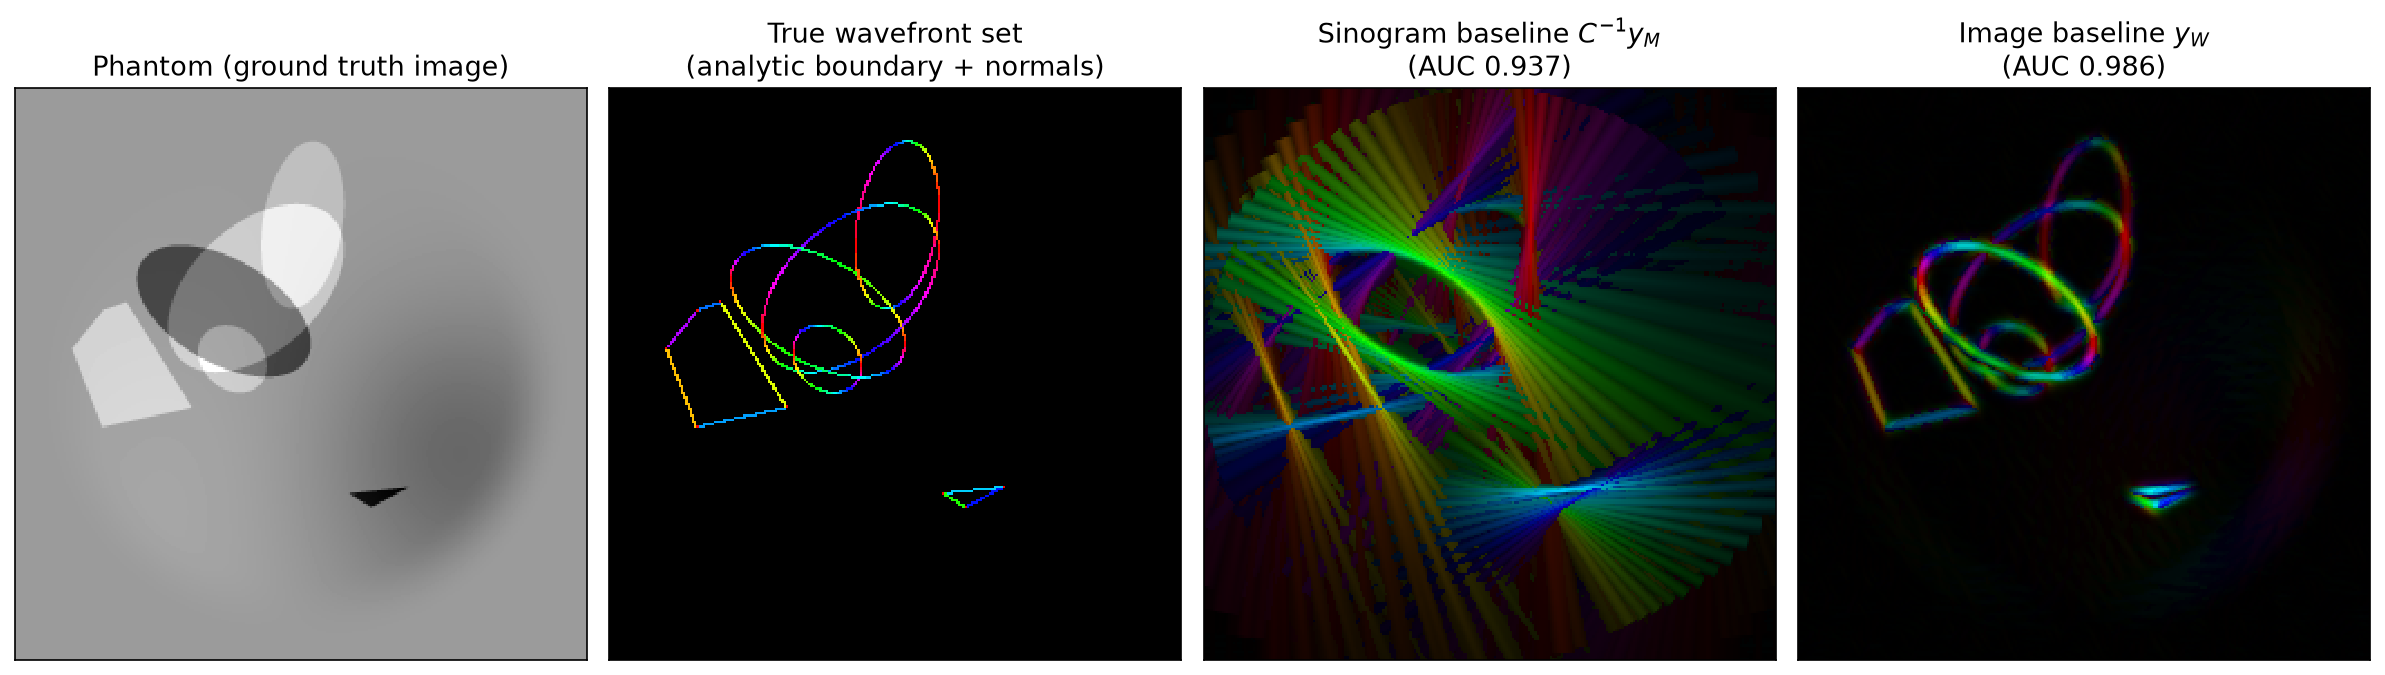
\includegraphics[width=\linewidth]{assets/fig_val_inputs.png}

  \vspace{0.2em}
  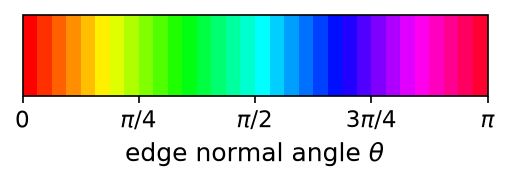
\includegraphics[width=0.3\linewidth]{assets/theta_legend.png}

  \small
  Held-out phantom. $C^{-1}y_M$ smears every edge point along its tangent line. $y_W$ is sharp in $x$ but blurry in angle.
\end{frame}

\begin{frame}{Validation Example: LPD Output And Thin Ridges}
  \centering
  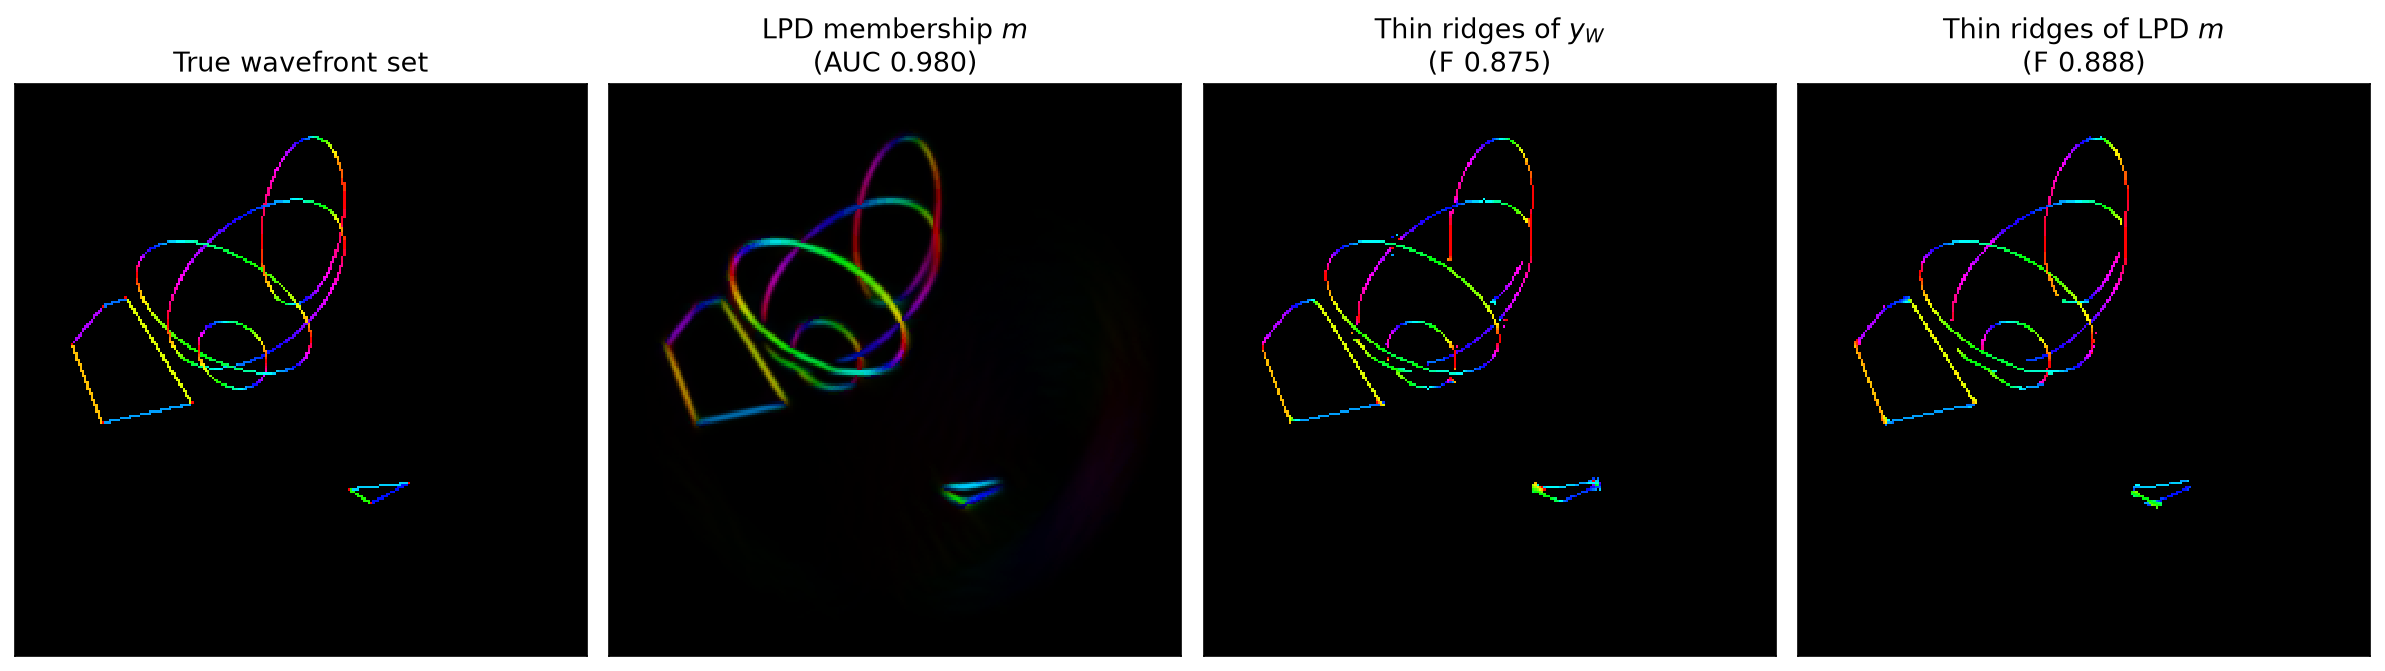
\includegraphics[width=\linewidth]{assets/fig_val_outputs.png}

  \vspace{0.2em}
  \small
  Without a contrast output, the thin ridges of $m$ are slightly better than those of $y_W$.
  (Step 1500; AUC for this sample, F over the validation set.)
\end{frame}

\begin{frame}{Validation Summary}
  \begin{columns}[T]
    \begin{column}{0.50\linewidth}
      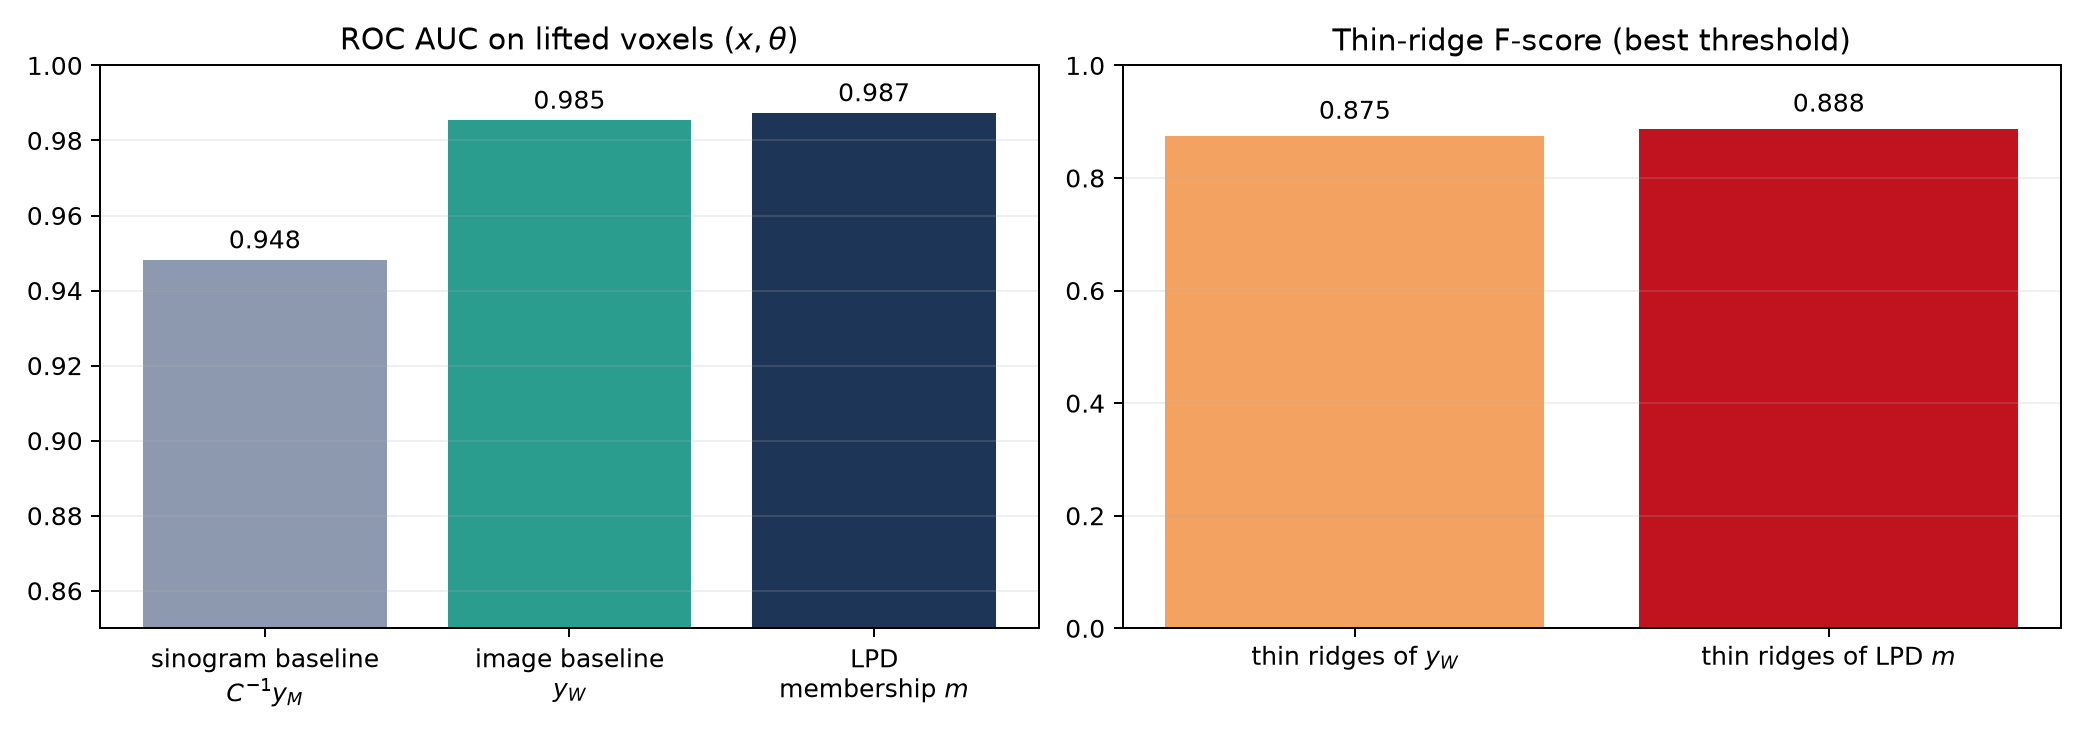
\includegraphics[width=\linewidth]{assets/metrics.png}
    \end{column}
    \begin{column}{0.48\linewidth}
      \small
      Mean over the 8 validation phantoms ($256^2$, $K=32$, step 1500):

      \vspace{0.3em}
      {\footnotesize
      \begin{tabular}{@{}lccc@{}}
        \toprule
         & $C^{-1}y_M$ & $y_W$ & LPD $m$ \\
        \midrule
        ROC AUC & 0.948 & 0.986 & \textbf{0.987} \\
        AP & 0.18 & 0.37 & \textbf{0.78} \\
        hard-neg.\ AUC & 0.865 & 0.919 & \textbf{0.960} \\
        ridge F & -- & 0.875 & \textbf{0.888} \\
        ridge $F_x$ & -- & 0.975 & 0.976 \\
        \bottomrule
      \end{tabular}}

      \vspace{0.5em}
      The network ranks voxels best, with far fewer confident false positives (AP); its thin ridges are now on par with those of $y_W$.
    \end{column}
  \end{columns}
\end{frame}

\begin{frame}{Loss Convergence And Metric Evolution}
  \centering
  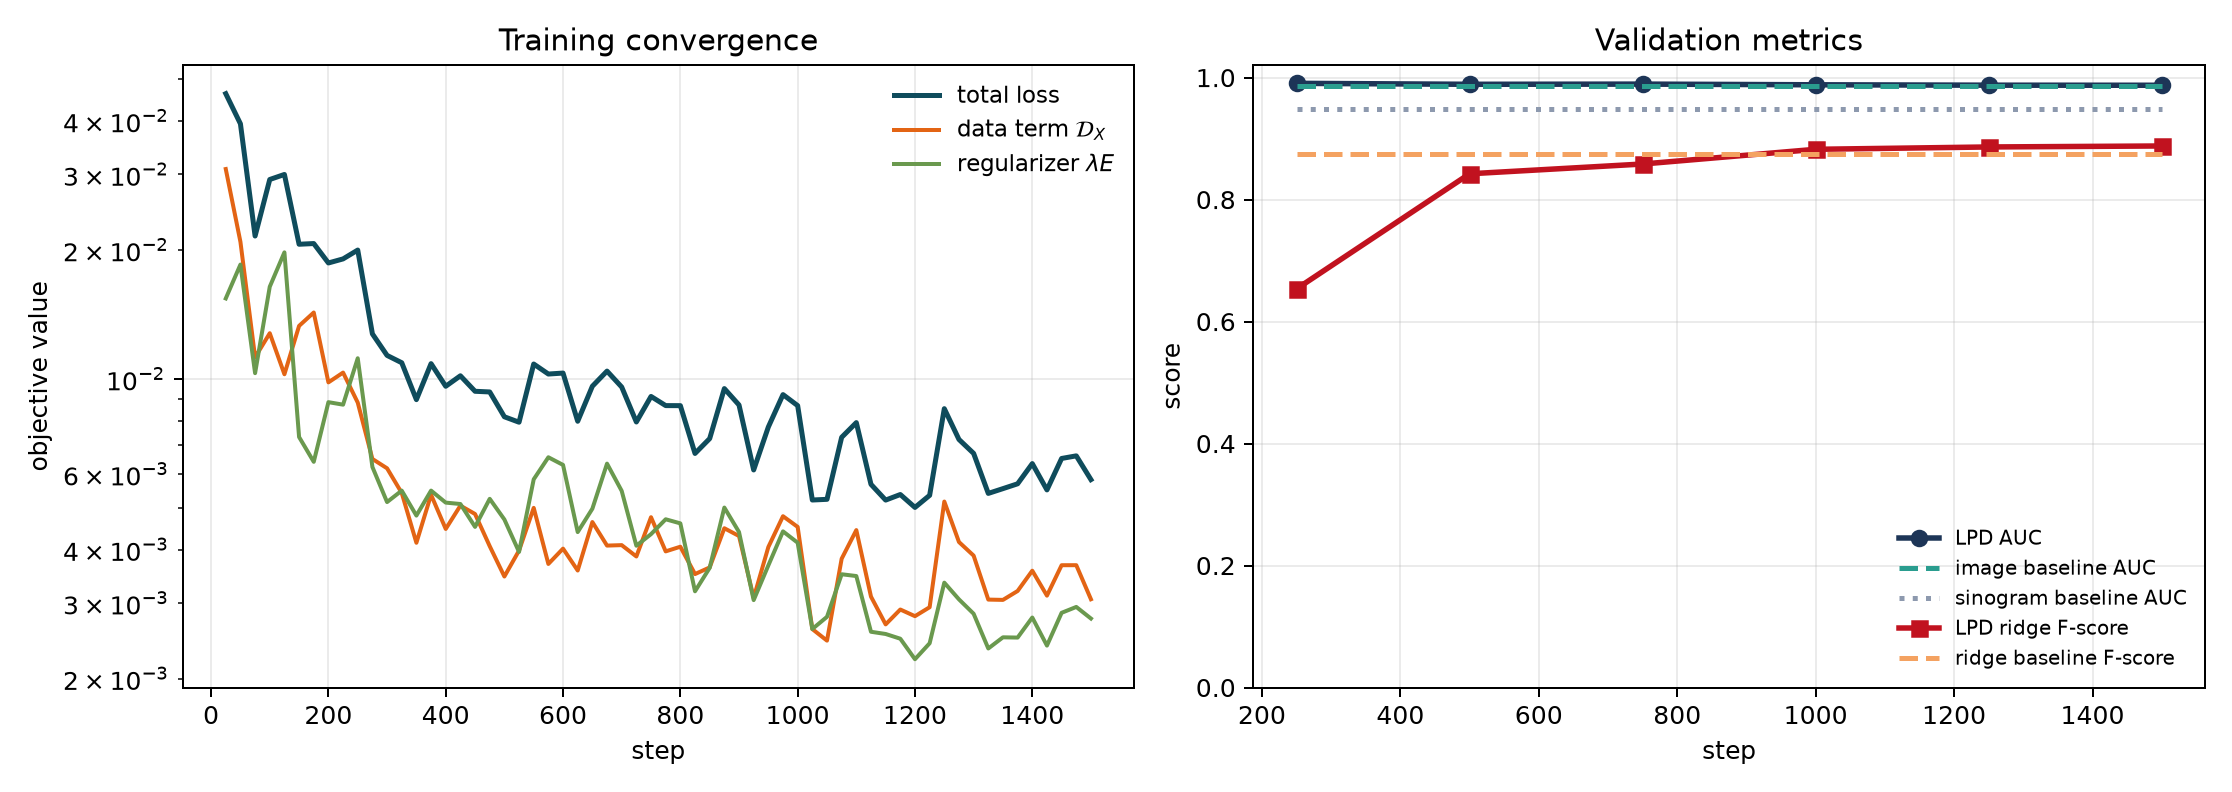
\includegraphics[width=0.95\linewidth]{assets/convergence.png}
  \vspace{0.3em}

  \small $\mathcal D_X$ converges quickly. AUC is near its final value at the first check (step 250); ridge F improves until about step 1000 and then passes $y_W$.
\end{frame}

\begin{frame}{What Happens Inside The 5 LPD Iterations}
  \centering
  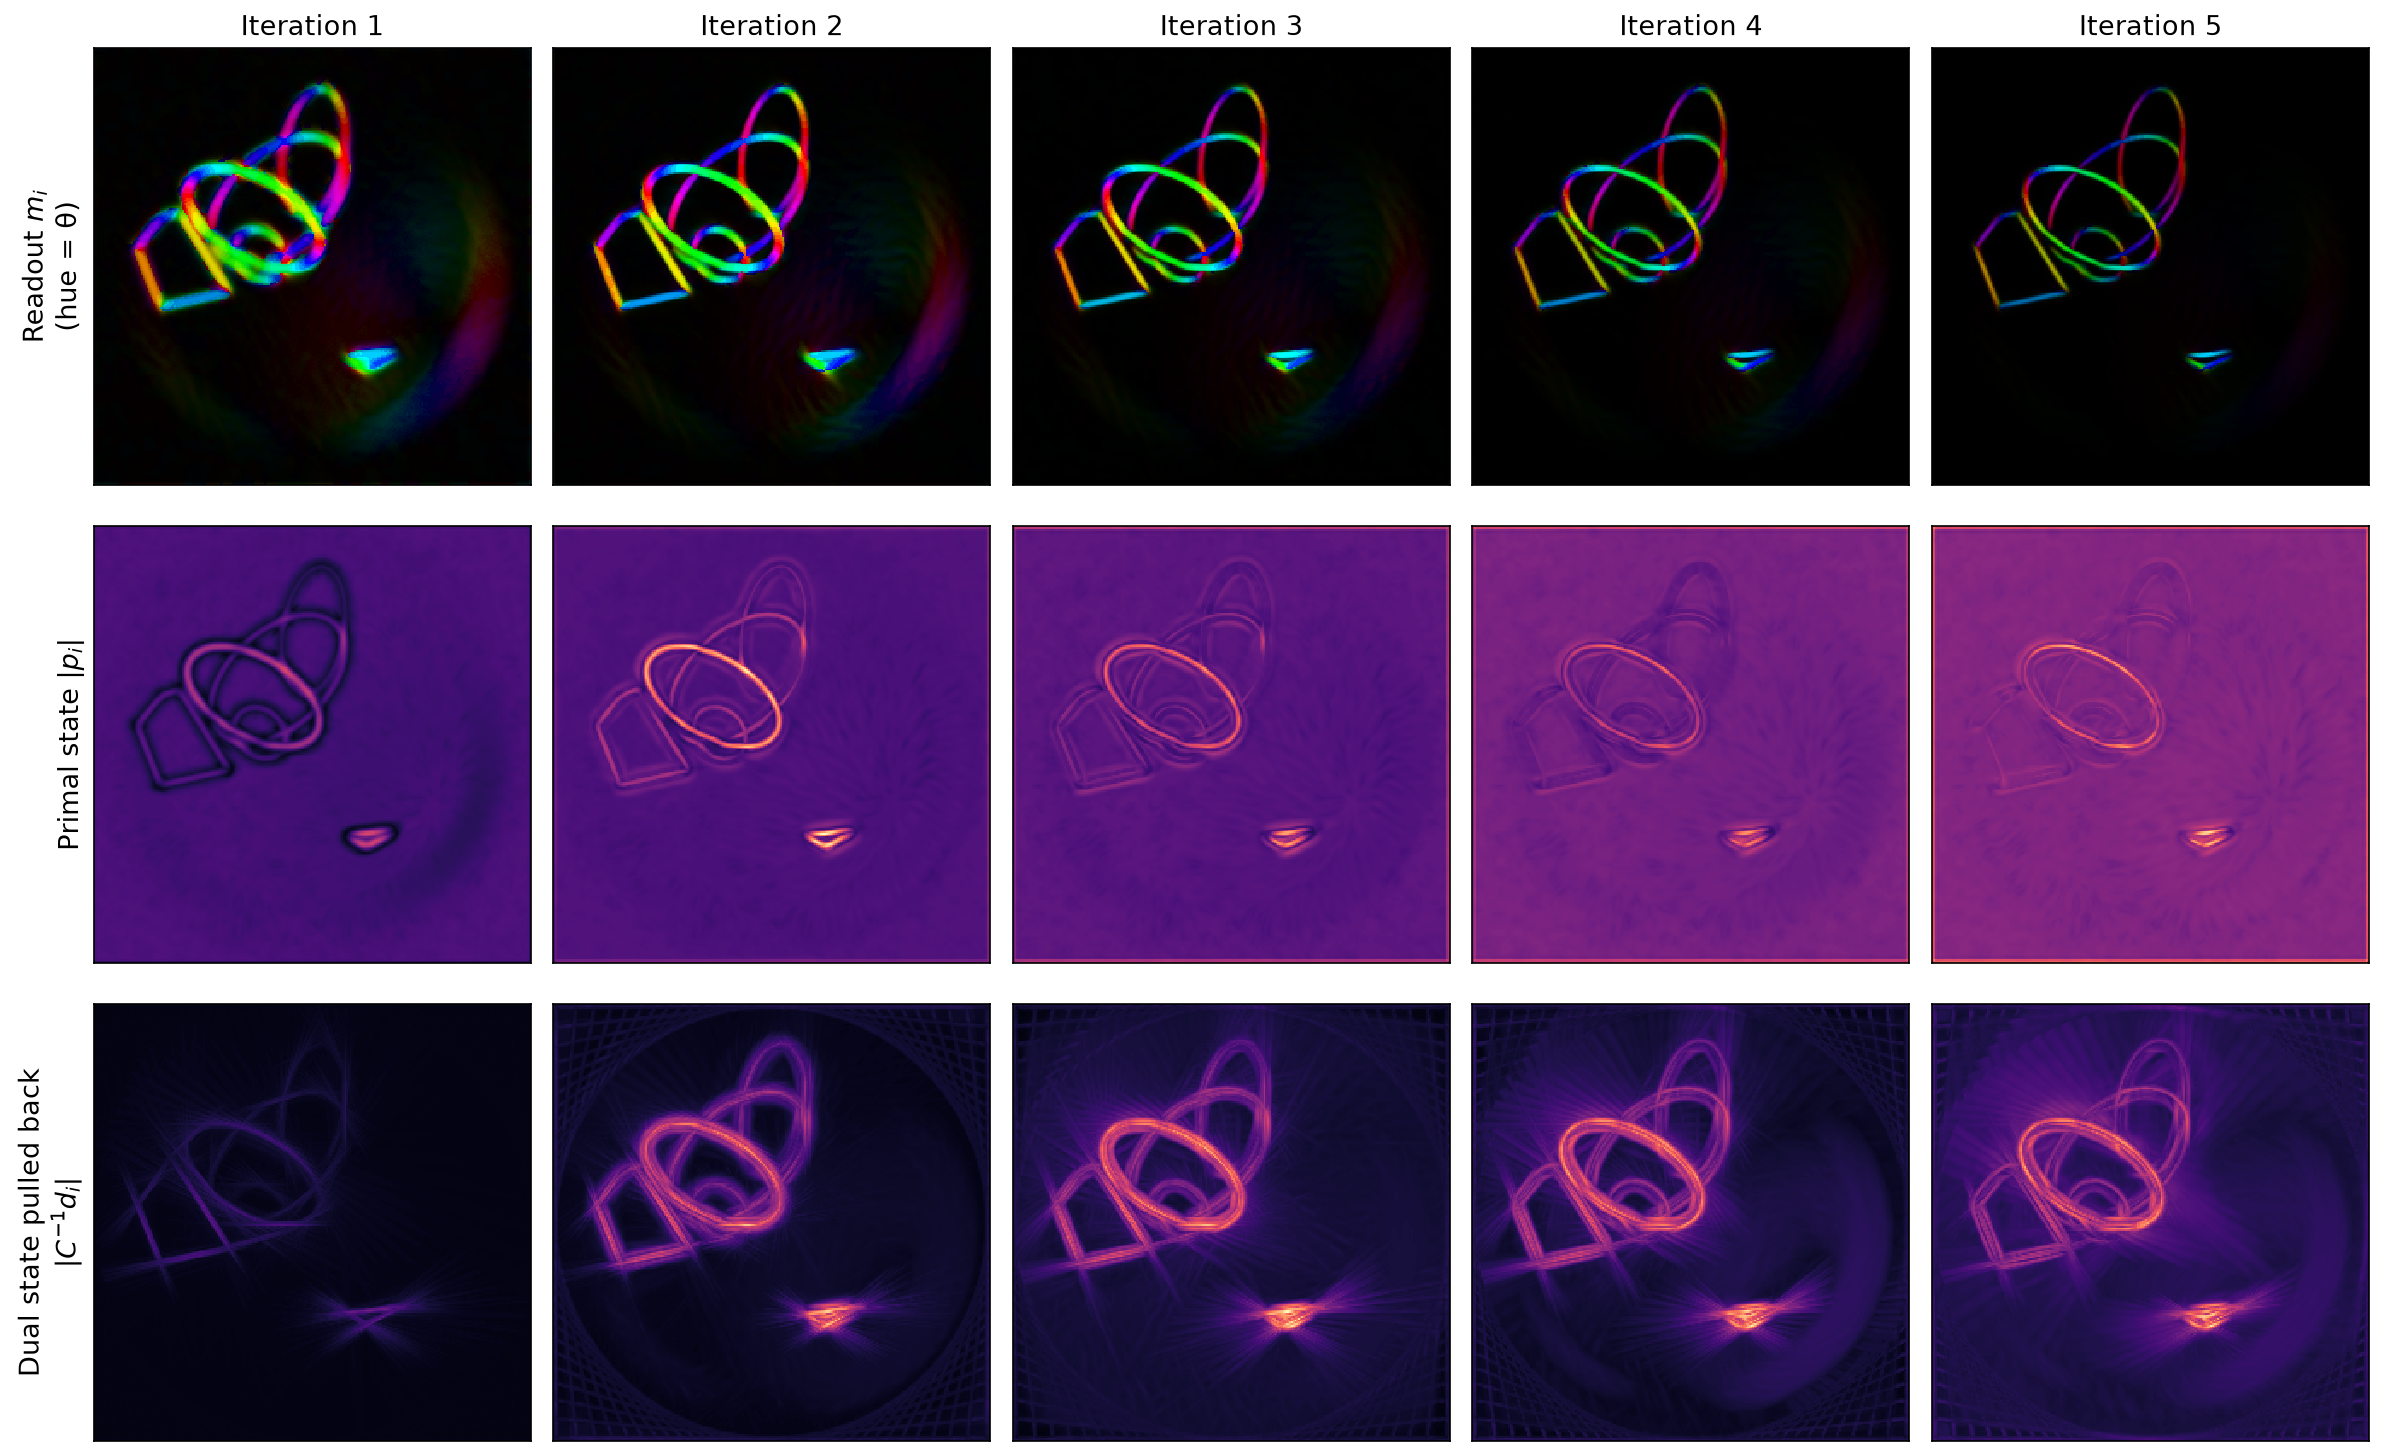
\includegraphics[height=0.66\textheight]{assets/fig_iterations.png}

  \small Iterations 1--2: hazy readout (each panel scaled to its own max). Later iterations suppress the background, and the curves sharpen up to iteration 5.
  The dual state accumulates the streaks of $C^{-1}y_M$.
\end{frame}

\begin{frame}{How Well Does The Output Explain The Data?}
  \centering
  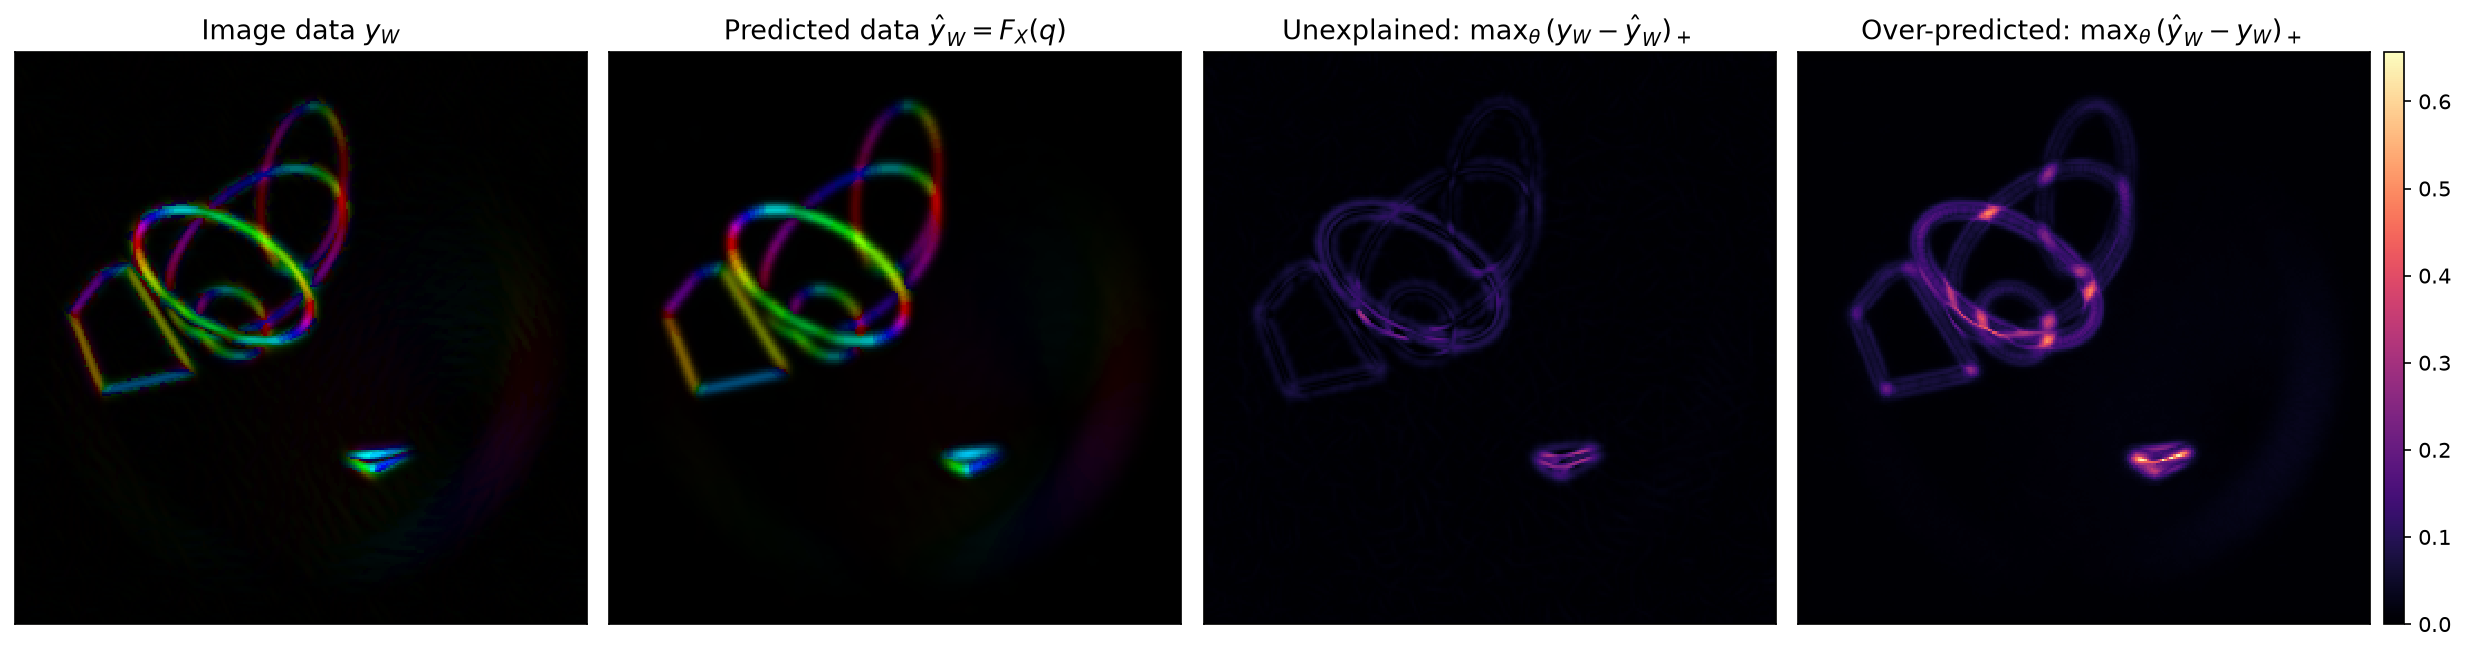
\includegraphics[width=\linewidth]{assets/fig_datafit.png}

  \vspace{0.2em}
  \small
  $\hat y_W=F_X(q)$. Remaining misfit: \emph{over}-prediction where two edges cross and on the small triangle; little \emph{under}-prediction, mainly along close parallel edges.
\end{frame}

\begin{frame}{Learned Outputs And Where The Prior Pays}
  \centering
  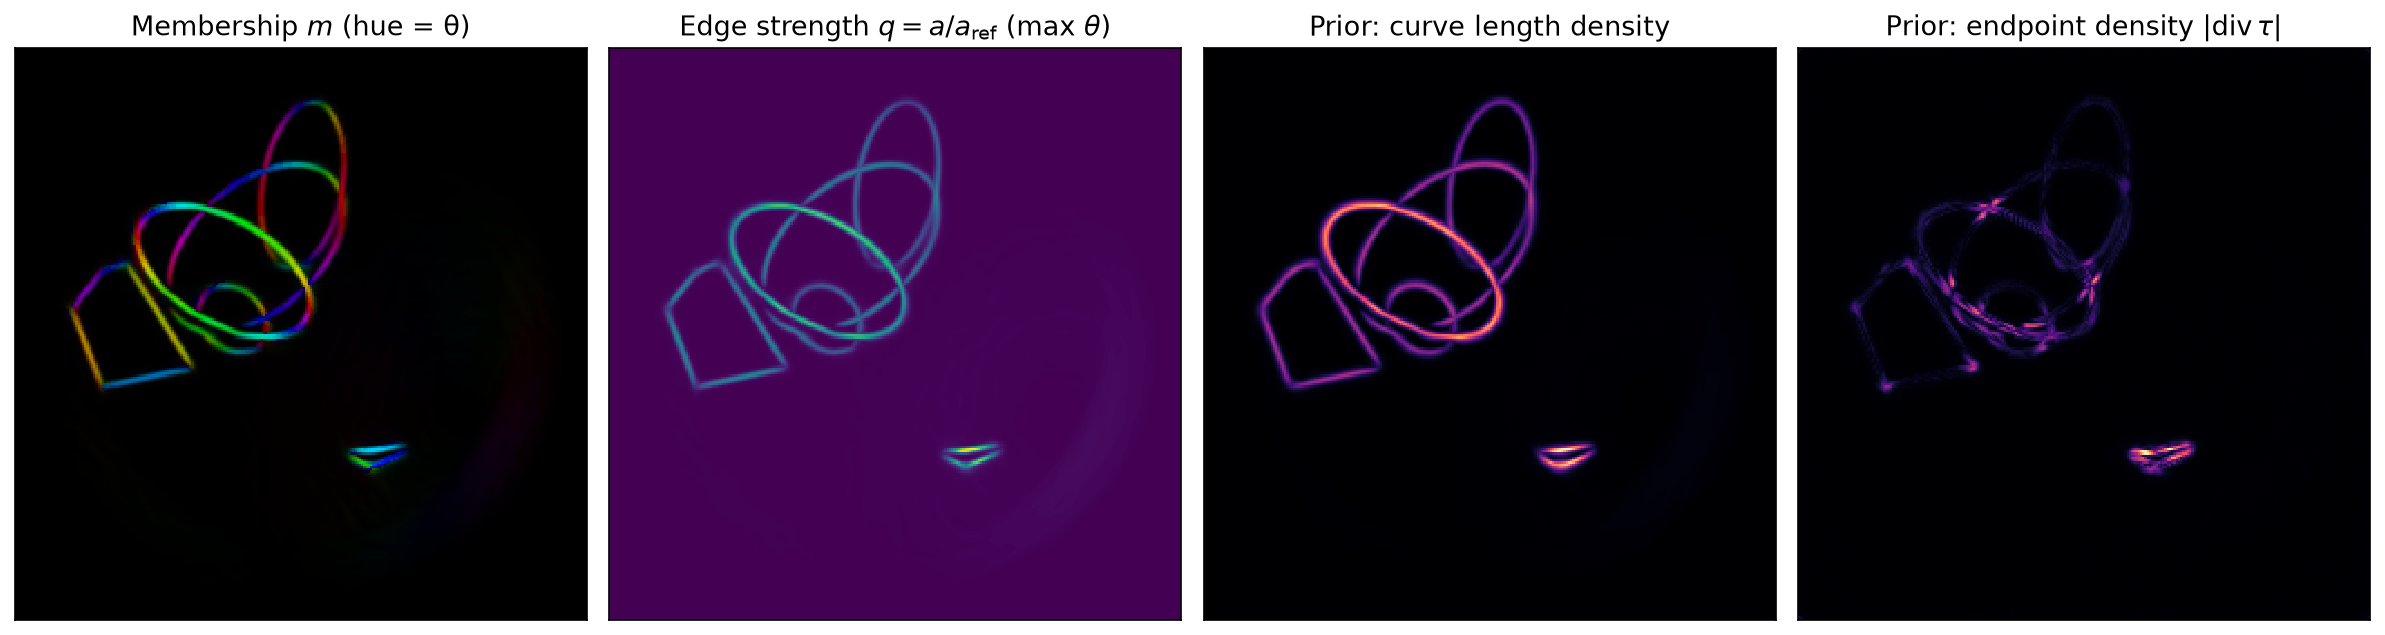
\includegraphics[width=\linewidth]{assets/fig_outputs_prior.png}

  \vspace{0.2em}
  \small
  $q=a/a_\mathrm{ref}$ measures edge strength: weak edges get a small $q$ (and $m$), and $\lambda$ sets the weakest edge that is kept.
  The length cost concentrates on the true curves; the endpoint cost at corners and crossings.
\end{frame}

\begin{frame}{Walnut Data: Qualitative Results}
  \centering
  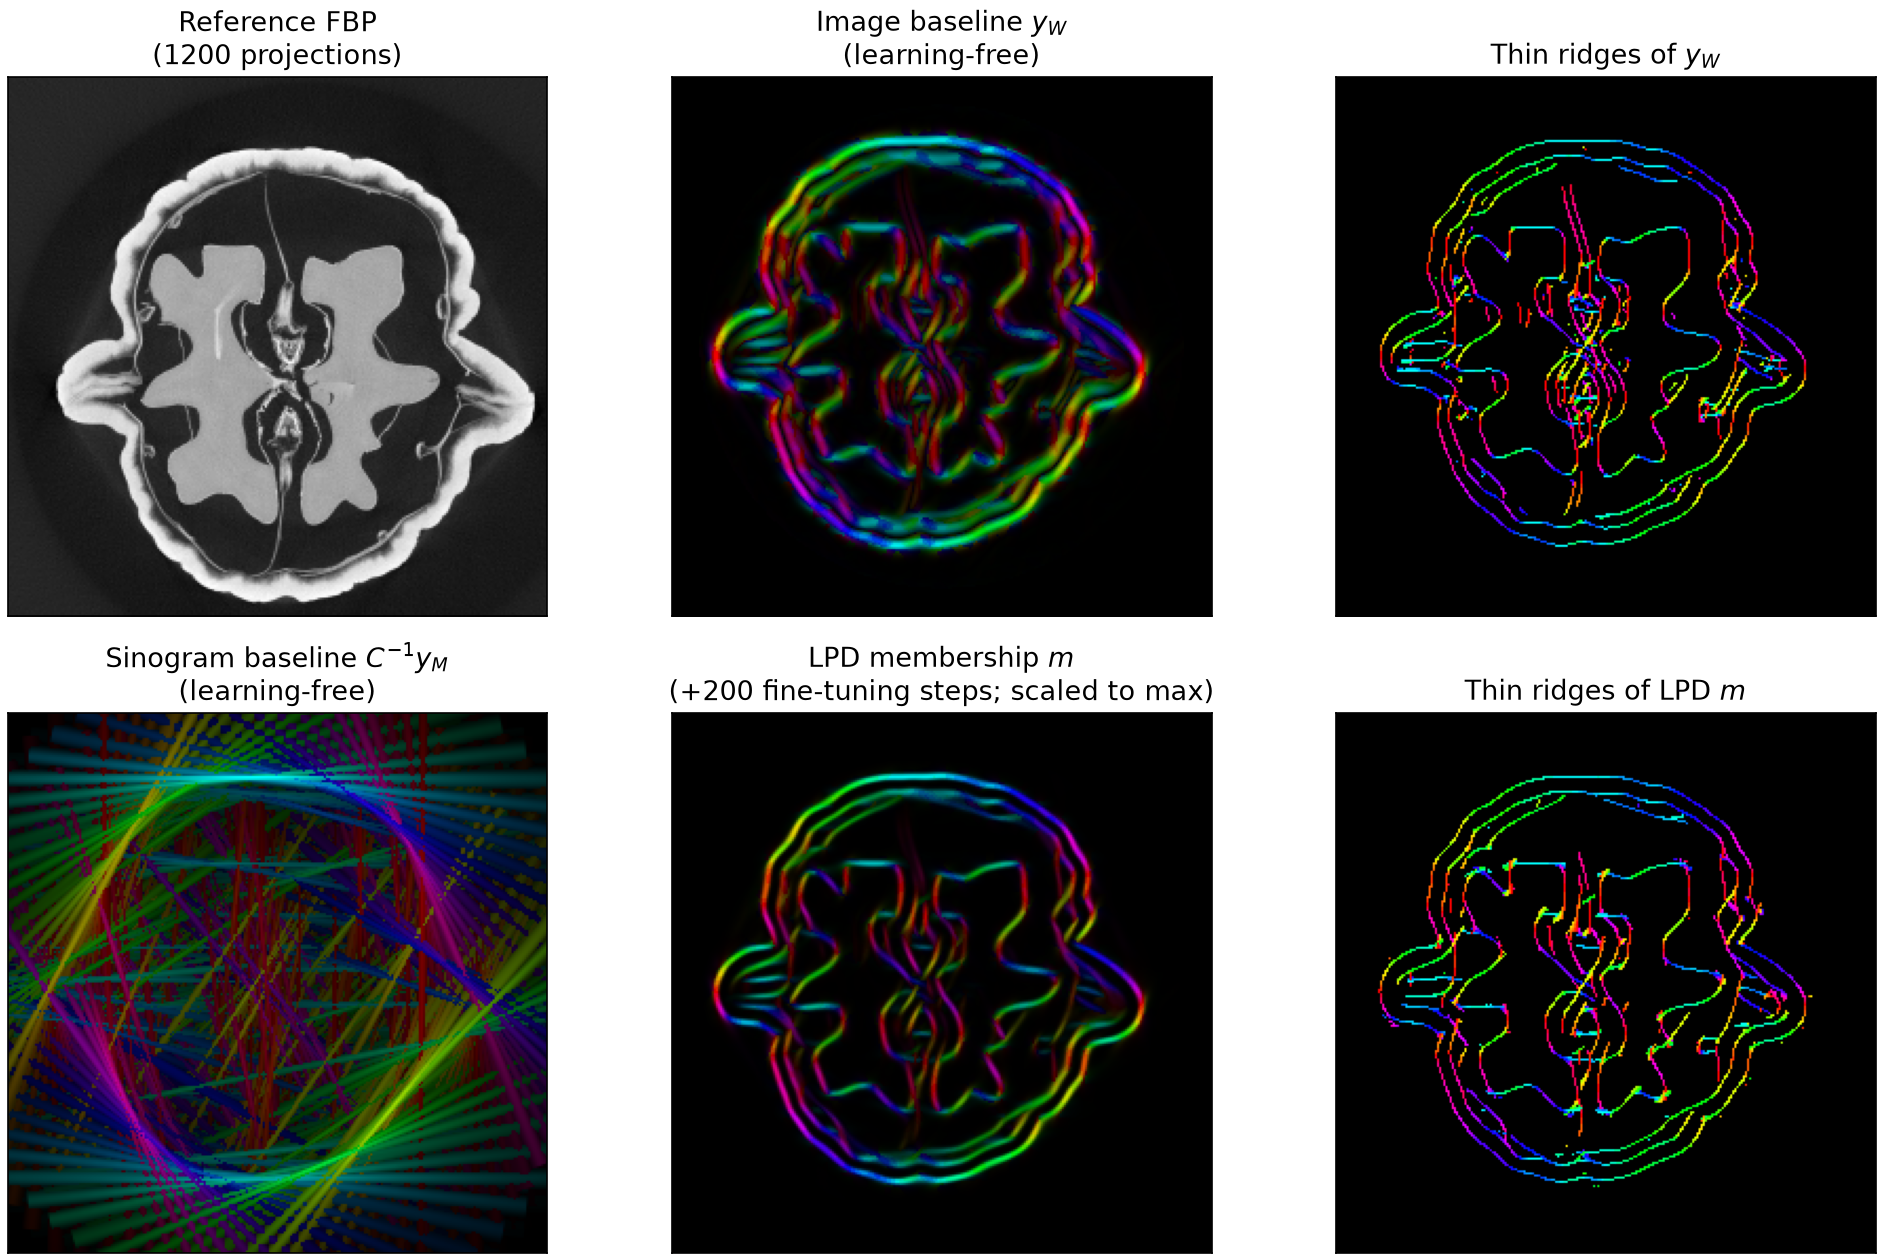
\includegraphics[height=0.62\textheight]{assets/fig_walnut.png}

  \footnotesize Measured data, no ground truth. Trained on synthetic phantoms, then 200 unsupervised fine-tuning steps on the walnut (5 min).
  97\% of the ridge pixels of $m$ lie within 2\,px of a ridge of $y_W$, and they cover 91\% of the ridges of $y_W$. Fewer spurious streaks, noisier orientations at junctions: \textbf{not yet better than $y_W$}.
\end{frame}

\begin{frame}{Walnut: The Lifted Fields $a$, $b$, $c$}
  \centering
  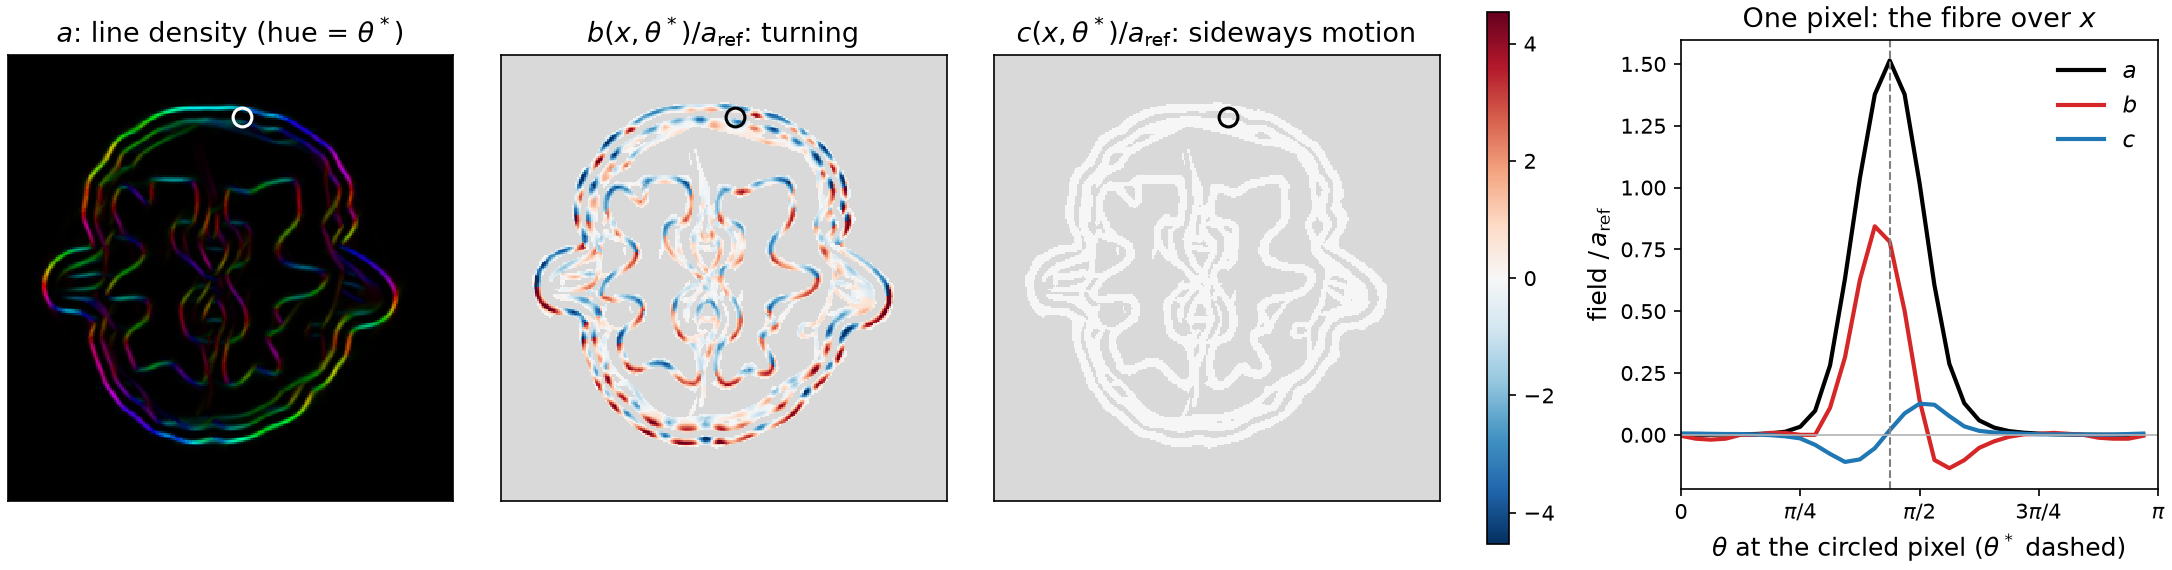
\includegraphics[width=\linewidth]{assets/fig_walnut_fields.png}

  \vspace{0.2em}
  \footnotesize
  $a,b,c$ (and $m$) are fields on $(x,\theta)$, $32$ angles per pixel; not a distribution over $\theta$ (crossings can have two peaks).
  Maps: $a$ as max over $\theta$ with hue $\theta^*=\arg\max_\theta a$; $b,c$ are signed, so they are read out \emph{at} $\theta^*$.
  $c\approx0$ ($|c|\lesssim0.04\,a_\mathrm{ref}$): $\theta$ follows the curve normal. $b$ peaks at $\theta^*$ on the centre line (right), so $b/a\approx\kappa$; its sign alternates along the wavy shell.
\end{frame}

\begin{frame}{Evaluating On Real Data (Plan)}
  \begin{itemize}
    \item No ground truth. Today: qualitative, plus agreement with $y_W$.
    \item \textbf{Pseudo ground truth} from the 1200-projection reference, using a slower, \emph{independent} method:
      \begin{itemize}
        \item a multi-scale shearlet/curvelet decay test (Thm.~5.1), or
        \item a long non-learned PDHG solve of the MAP problem.
      \end{itemize}
    \item Evaluate the network on \textbf{reduced data}: fewer angles, more noise.
    \item \textbf{Caveat:} the pseudo ground truth must not be the same detector as a baseline.
  \end{itemize}
\end{frame}

\begin{frame}{Compute Cost: Memory And Run Time}
  \centering
  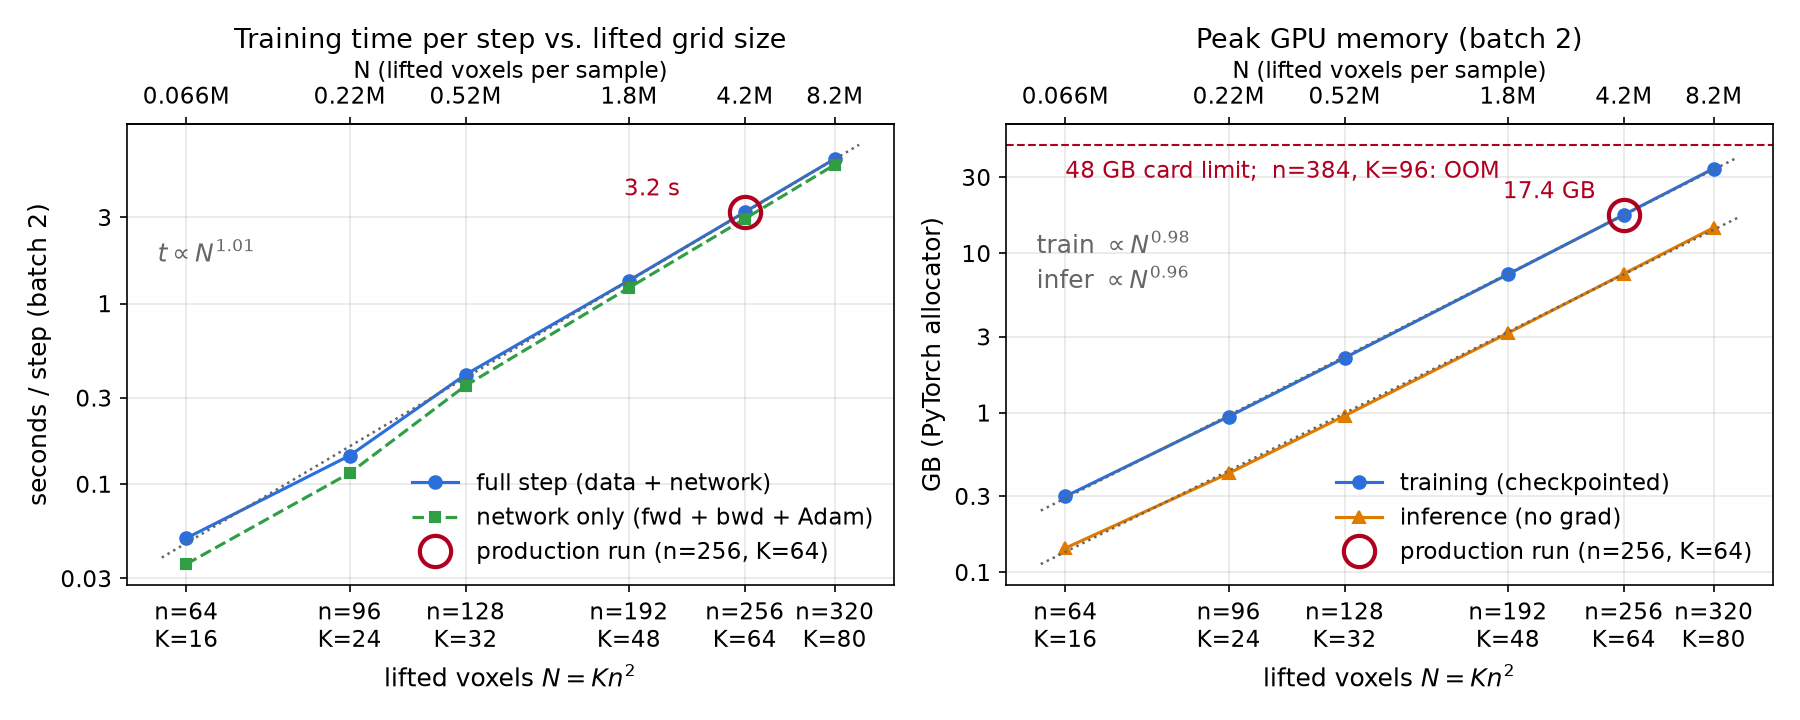
\includegraphics[width=0.70\linewidth]{assets/fig_scaling.png}

  \small
  \begin{itemize}
    \item Time and memory scale \textbf{linearly} with $N=Kn^2$ (fits $N^{1.01}$, $N^{0.98}$).
    \item $n=256$, $K=64$, batch 2 (RTX 6000 Ada, 48\,GB): 3.2\,s/step, 17.4\,GB, 1.4\,h for 1500 steps. The results here use $K=32$: 1.8\,s/step, 45\,min.
    \item Largest grid that fits: $n=320$. Only 286k parameters; memory is the 3D activations.
  \end{itemize}
\end{frame}

\begin{frame}{Current Limitations}
  \begin{itemize}
    \item \textbf{Forward-model misfit:} edges add before $|\cdot|$ at crossings; close parallel edges; smooth intensity variation.
    \item \textbf{Dense angles needed:} sparse-view tomography remains open.
    \item \textbf{Data term on $y_W$, not $y_M$:} the sinogram-side term ($\hat y_M=\mathcal R_t C q$) is implemented but unused here.
    \item \textbf{$m$ measures edge strength:} $\lambda$ sets the weakest edge that is detected; contrast-invariant membership needs local normalization of $y_W$.
    \item \textbf{Angular resolution:} at $K=64$ the ridge F drops to $0.77$ (vs $0.89$ at $K=32$); not yet understood.
  \end{itemize}
\end{frame}

\begin{frame}{Useful Next Steps}
  \begin{itemize}
    \item Quantitative real-data evaluation with an independent pseudo ground truth.
    \item Multi-scale data terms, to separate singularities from smooth texture.
    \item Local normalization of $y_W$, if membership should not depend on contrast.
    \item Sparse-angle analyzers, where the prior must do more of the work.
    \item Exact $SE(2)$ group convolutions on the primal side.
  \end{itemize}
\end{frame}

\begin{frame}{Takeaways}
  \begin{itemize}
    \item Microlocal geometry plus a learned primal-dual network maps sinogram data to a wavefront set on $(x,\theta)$, without a regularized or learned reconstruction.
    \item The regularizer is a convex prior with five desirable properties for curves.
    \item Synthetic validation: LPD $m$ ranks best (AUC $0.987$, AP $0.78$, hard-negative AUC $0.960$) and its thin ridges match $y_W$ (F $0.888$ vs $0.875$).
    \item One output field $(a,b,c)$, no contrast: the MAP objective is convex, and $b$ carries the curvature.
    \item The remaining gap: thin-curve extraction and real-data robustness.
  \end{itemize}
\end{frame}

% ---------------------------------------------------------------------------
\appendix

\begin{frame}{Backup: Why There Is No Contrast Output}
  Earlier design: $q=J\,m(a)$ with a learned contrast $J\in(0,J_{\max})$.
  \begin{itemize}
    \item $(J,m)$ is not identifiable from $q$, and the prior charges $a$ but not $J$: a smaller $a$ with a larger $J$ fits equally well at lower prior cost.
    \item $J_{\max}=1$: $J$ saturates ($J\ge0.95$ on 99\% of detected voxels). $J_{\max}=4$: the network escapes the prior and collapses (AUC 0.49).
    \item The saturating $m$ made the objective non-convex.
  \end{itemize}
  Now $q=a/a_\mathrm{ref}$: one field, convex objective, and $a$ measures edge strength.
\end{frame}

\begin{frame}{Backup: $y_W$ Is A Fixed Linear Map Of $y$, Then $|\cdot|$}
  \[
    W_\theta*\mathrm{FBP}\,y=R^\#\bigl((RW_\theta)*_s\Lambda y\bigr)
  \]
  \begin{itemize}
    \item $R$: ray transform; $R^\#$: backprojection (its adjoint).
    \item $\mathrm{FBP}\,y=R^\#(\Lambda y)$ (up to a constant), with $\Lambda$ the ramp filter in $s$.
    \item $*_s$: 1-D convolution in $s$, separately for each angle $\varphi$.
    \item Fourier slice / intertwining: $R(W*f)=(RW)*_s Rf$, hence
      \[
        W*R^\#g=R^\#\bigl((RW)*_s g\bigr).
      \]
    \item With $g=\Lambda y$: $y_W$ is a fixed linear map of $y$ (1-D filters $RW_\theta$ over all angles), followed by $|\cdot|$.
  \end{itemize}
\end{frame}

\end{document}
